\documentclass[paper-main.tex]{subfiles}


\begin{document}

% the webcam method
% how to analyse video, python OpenCV2

Continuous wave searches look for signals which are close to monochromatic. 
In this section we consider a simple sinusoidal tone; a constant note. 
As described in Section~\ref{sec:ifo}, the audio is played through a speaker fixed to the back of one of the mirrors.


The intensity of the interference pattern is measured at a single point on the screen using a commercial USB webcam placed to view the screen (see Fig.~\ref{fig:ifo_schematic_webcam}). 
The webcam's sample rate is $30\,{\rm Hz}$, which limits the spectral content of observable signals to below $15\,{\rm Hz}$, the Nyquist frequency.
A tone under $15\,{\rm Hz}$ is played through the speaker for a minute and the interference pattern recorded with the webcam. 


The resulting data is a video capture of the whole interference pattern. 
As only the frequency of the interference ring motion is needed, we take data from a single off-centre pixel indicated by the red dot in Fig.~\ref{fig:interference_pattern}. 
We take the green-channel of the video as an approximation to the total intensity as the laser produces monochromatic green light (at $532\,{\rm nm}$).


As an initial inspection, we play the timeseries of the intensity using the \textbf{io.wavfile.write} function from the Scipy~\cite{scipy} package in Python~\cite{python}. 
The two tones sound similar by ear and don't produce any noticeable beating. 
The result is quantified in Fig.~\ref{fig:webcam_spectrum}. 
A tone of $2.09\,{\rm Hz}$ is played through the speaker and the data recorded via webcam. 
Figure~\ref{fig:webcam_spectrum} shows the Fourier transform of the recording. 
We measure a peak amplitude at $(2.099\pm 0.008)\,{\rm Hz}$ \han{[James: I added in that this is the $1\sigma$ uncertainty, is that correct?] (where the error represents the $1\sigma$ uncertainty).}
The demonstration is able to recover a single frequency tone to within two standard deviations. 
%We played this time series of intensity over time as an audio recording using the \textbf{io.wavfile.write} function from the Scipy~\cite{scipy} package in Python~\cite{python}. 
%The two tones played together sound similar and don’t produce any noticeable beating.
%To quantify the precision, we recorded a signal from an injected tone of $2.09\,{\rm Hz}$. 
%From the Fourier transform shown in Figure~\ref{fig:webcam_spectrum}, we measured a peak amplitude at $(2.099\pm 0.008)\,{\rm Hz}$, a result within two standard deviations. 
%The experiment is able to recover a single tone confidently. 
%This showed that the experiment observes a single tone confidently.

\begin{figure}
	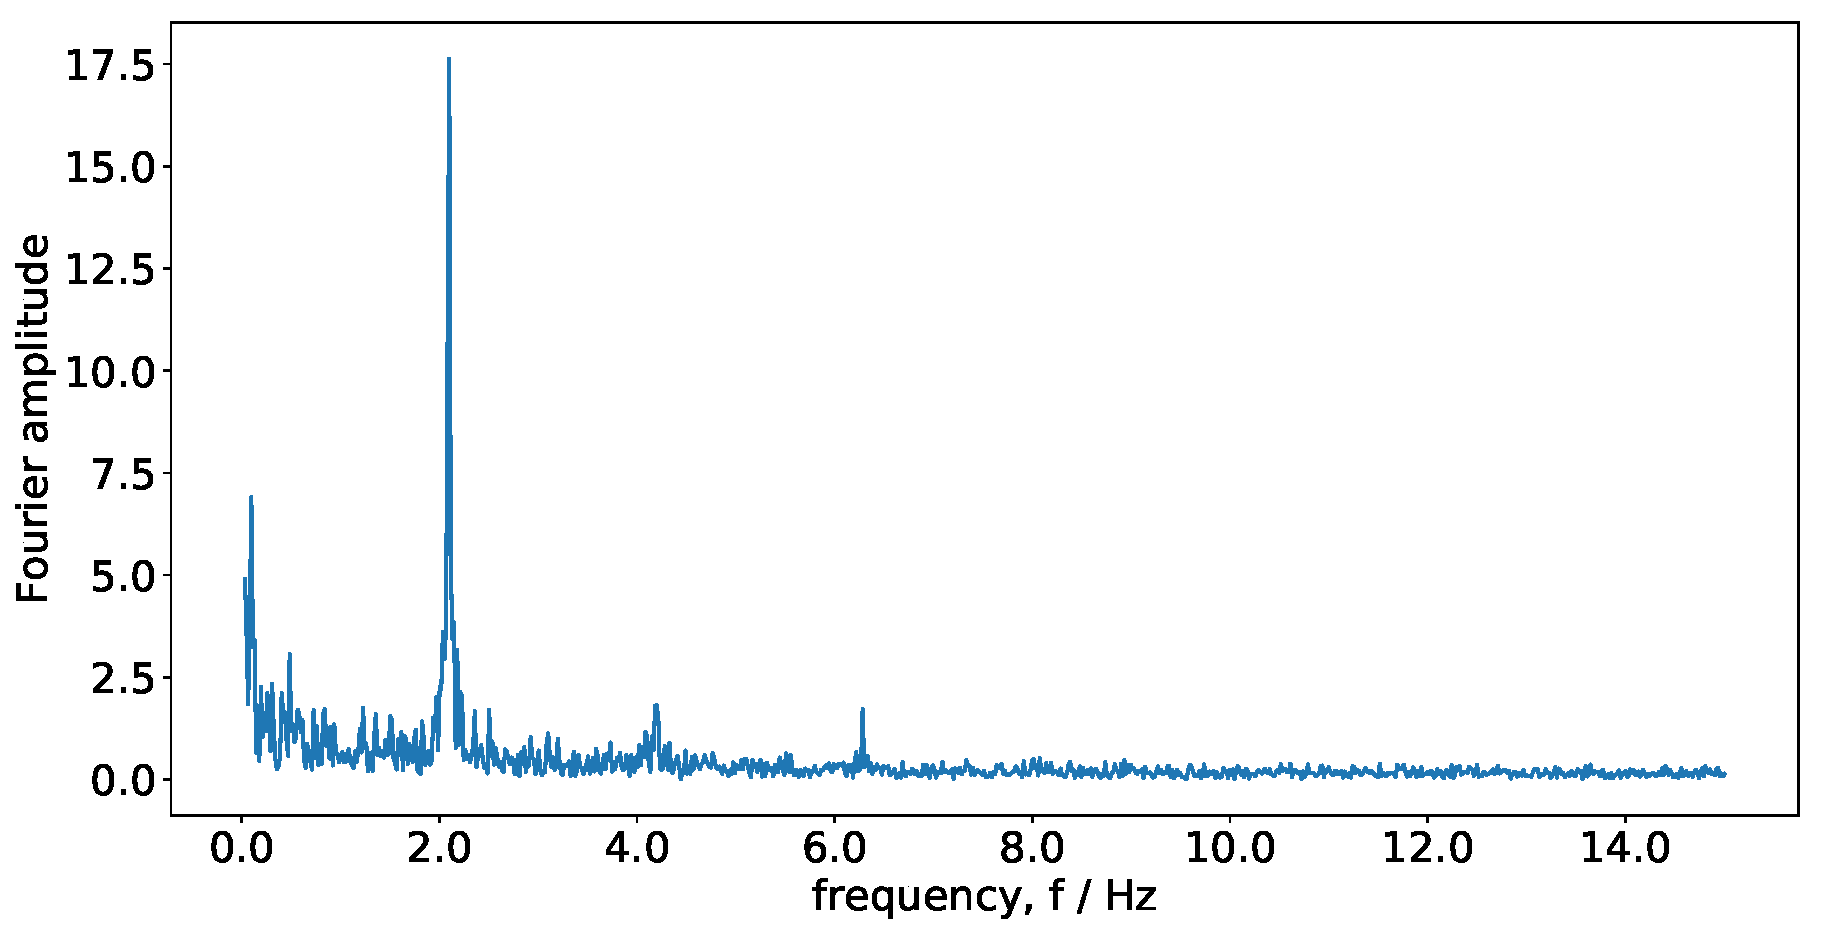
\includegraphics[width=.49\textwidth]{figures/webcam_expt_4_0209-cropped.pdf}
	\caption{\label{fig:webcam_spectrum}
Single injected tone results. 
The Fourier amplitude of the intensity timeseres recorded by webcam. 
The frequency of the injection is $2.09\,{\rm Hz}$. 
The recovered frequency peak is at $(2.099\pm 0.008)\,{\rm Hz}$. 
%The peak (with amplitude $17.5$) has a frequency was measured at $(2.099\pm 0.008) \mathrm{Hz}$. The actual maximum is achieved at $0\,{\rm Hz}$, but corresponds to the signal having a non-zero average value, so we don’t display or consider it.
}
	
\end{figure}


\end{document}

\begin{comment}
As described in Section~\ref{sec:introduction}, continuous gravitational wave searches look for near monochromatic signals. 
The audio analogue of this is a simple sinusoidal tone; a constant note.


The intensity of the interference pattern is measured at a single point on the screen using a commercial USB webcam placed to view the screen (see Figure~\ref{fig:ifo_schmatic_webcam}). 
The webcam's sample rate is $30\,{\rm Hz}$, which limits the spectral content of observable signals to below 15Hz, the Nyquist frequency.
A tone under $15\,{\rm Hz}$ is played through the speaker for a mintue and the interference pattern recorded with the webcam. 


The data is taken from a single off-centre pixelm, indicated by the red dot in Figure~\ref{fig:interference_pattern}. 
We take the green-channel of the video as an approximation to the total intensity as the laser is monochromatic green light (at $532\,{\rm nm}$).



We played this time series of intensity over time as an audio recording using the \textbf{io.wavfile.write} function from the Scipy~\cite{scipy} package in Python~\cite{python}. The two tones played together sound similar and don’t produce any noticeable beating.
To quantify the precision, we recorded a signal from an injected tone of 2.09Hz. From the Fourier transform shown in Figure~\ref{fig:webcam_spectrum}, we measured a peak amplitude at $(2.099\pm 0.008)\mathrm{Hz}$, a result within two standard deviations. This showed that the experiment observes a single tone confidently.

\begin{figure*}
	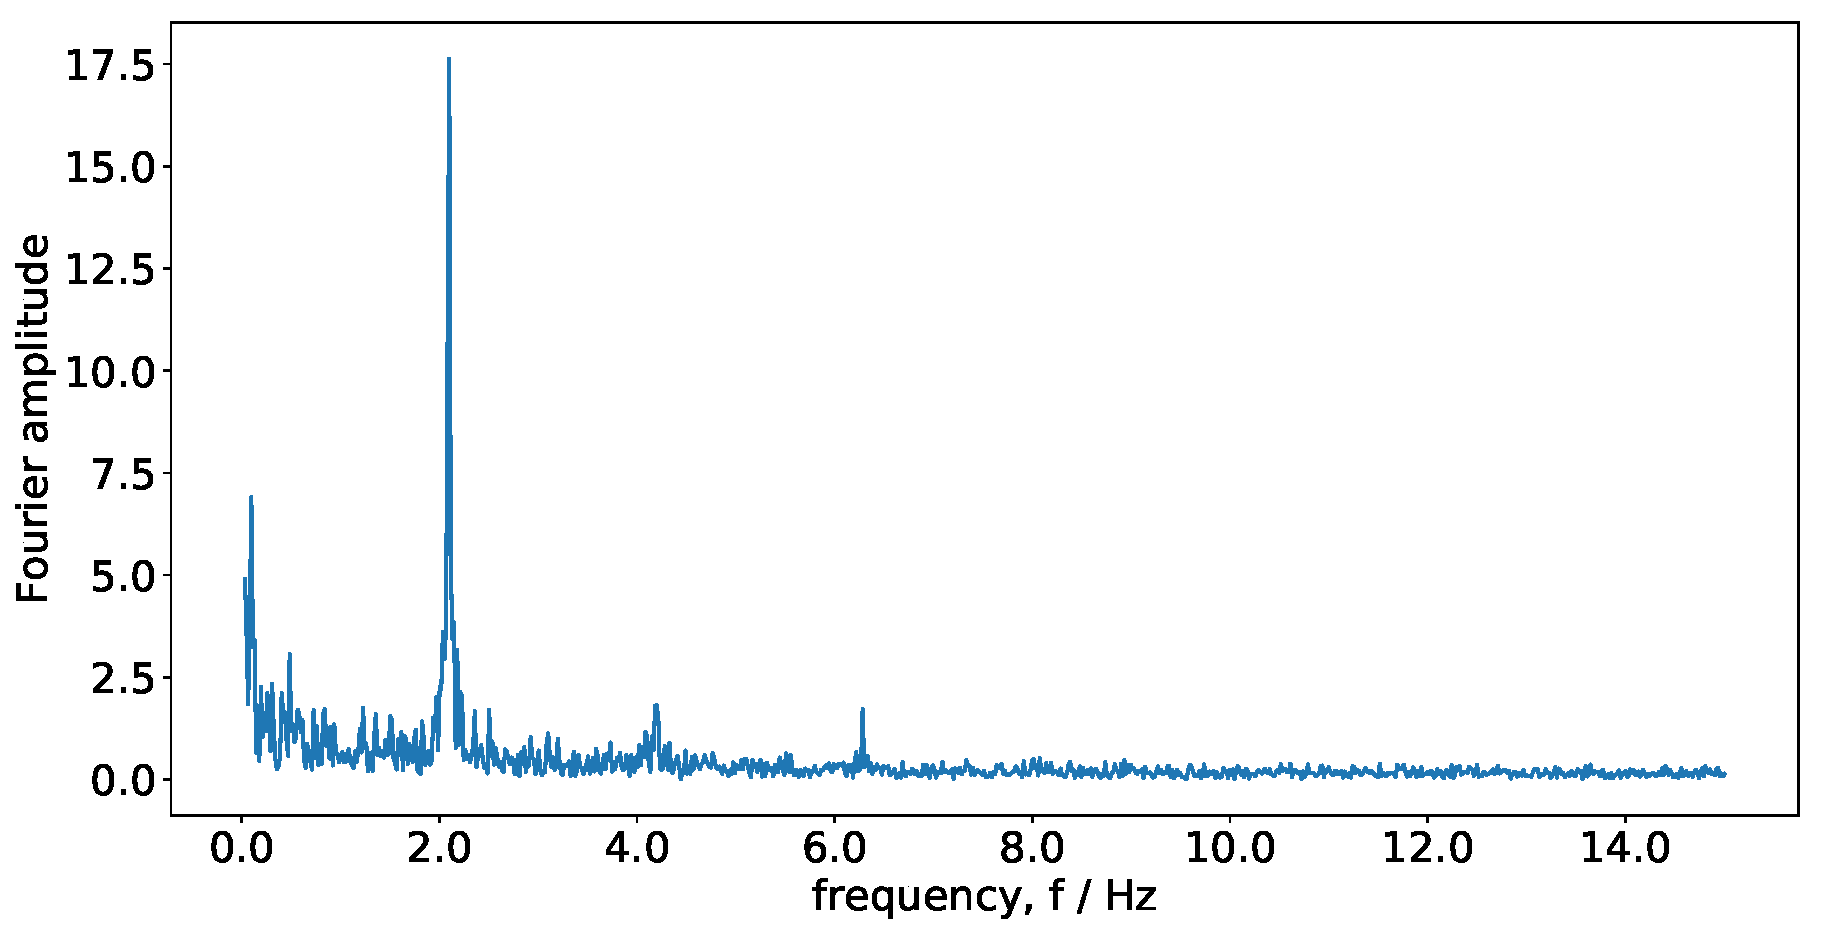
\includegraphics[width=\textwidth]{figures/webcam_expt_4_0209-cropped.pdf}
	\caption{Fourier amplitudes of intensity time series of interference pattern as captured by a webcam for an injected tone of 2.09Hz, the amplitude 17.5 peak was measured at $(2.099\pm 0.008) \mathrm{Hz}$. The actual maximum is achieved at 0Hz, but corresponds to the signal having a non-zero average value, so we don’t display or consider it.}
	\label{fig:webcam_spectrum}
\end{figure*}
\end{comment}
